% !TEX root = saveliev_physics_general_course_2.tex
%!TEX TS-program = pdflatex
%!TEX encoding = UTF-8 Unicode


\chapter[Dòng điện không đổi]{Dòng điện không đổi}\label{chap:5}
\chaptermark{Dòng điện không đổi}
\vspace{-0.3 cm}
\section{Dòng điện}\label{sec:5_1}

Nếu có một lượng điện tích khác không chuyển động xuyên qua một mặt phẳng tưởng tượng, một \textbf{dòng điện} (hay gọi tắt là \textbf{dòng}) được cho là chạy qua mặt phẳng đó. Dòng điện có thể chạy trong chất rắn (kim loại, chất bán dẫn), chất lỏng (chất điện giải) và chất khí (dòng điện chạy qua chất khí còn gọi là sự phóng điện). 

Để có dòng điện chạy qua, vật thể nhất định (hoặc môi trường nhất định) phải chứa các phần tử mang điện có thể di chuyển trong giới hạn của toàn bộ vật thể. Những phần tử đó được gọi là \textbf{hạt tải điện}. Đó có thể là electron hay ion hoặc cuối cùng là các hạt vĩ mô thừa điện tích (ví dụ như các hạt bụi hay giọt chất lỏng tích điện).

% A current is produced if there is an electric field inside a body. The charge carriers participate in the molecular thermal motion and, consequently, travel with a certain velocity $\vec{v}$ even in the absence of a field. But in this case, an identical number of carriers of either sign pass on the average in both directions through an arbitrary area mentally drawn in the body, so that the current is zero.

Dòng điện được sinh ra nếu có một điện trường bên trong vật thể. Các hạt tải điện tham gia vào chuyển động nhiệt phân tử và do đó chuyển động với một vận tốc nhất định $\vec{v}$ ngay cả khi không có trường. Nhưng trong trường hợp này, một lượng giống nhau các hạt tải điện dương hoặc âm truyền trung bình qua một vùng tùy ý được vẽ trong vật thể từ cả hai hướng, do đó dòng điện bằng không. Khi trường được bật lên, chuyển động có trật tự với vận tốc $\vec{u}$ được chồng lên chuyển động hỗn loạn của các hạt với vận tốc $\vec{v}$\footnote{Tương tự, trong dòng khí, chuyển động có trật tự được đặt chồng lên chuyển động nhiệt hỗn loạn của các phân tử.}. Do đó, vận tốc của các hạt sẽ là $\vec{v}+\vec{u}$. Vì giá trị trung bình của $\vec{v}$ (nhưng không phải của $v$) bằng không nên vận tốc trung bình của hạt là $\average{\vec{u}}$:
\begin{equation*}
    \average{\vec{v}+\vec{u}} = \average{\vec{v}} + \average{\vec{u}} = \average{\vec{u}}.
\end{equation*}
\noindent
Từ những gì đã nói ở trên, dòng điện có thể được định nghĩa là chuyển động có trật tự của các điện tích.

Một đặc tính định lượng của dòng điện là độ lớn của điện tích truyền qua bề mặt đang xét trong một đơn vị thời gian. Nó được gọi là \textbf{cường độ dòng điện} hoặc đơn giản hơn là \textbf{cường độ}. Chúng ta phải lưu ý rằng dòng điện về bản chất là dòng chuyển dời của các điện tích qua một bề mặt (so sánh với dòng chảy của chất lỏng, thông lượng năng lượng,...).

% A quantitative characteristic of an electric current is the magnitude of the charge carried through the surface being considered in unit time. It is called the \textbf{current strength}, or more often simply the \textbf{current}. We must note that a current is in essence a flow of a charge through a surface (compare with the flow of a fluid, energy flux, etc.).


Nếu điện tích $\deriv{q}$ được truyền qua một bề mặt trong thời gian $\deriv{t}$, thì cường độ dòng điện là
\begin{equation}\label{eq:5_1}
    I = \diff{q}{t}.
\end{equation}

\noindent
Dòng điện có thể được tạo ra do chuyển động của các điện tích dương hoặc điện tích âm. Sự dịch chuyển của một điện tích âm theo một hướng tương đương với sự dịch chuyển của một điện tích dương cùng độ lớn theo hướng ngược lại. Nếu dòng điện được tạo ra bởi các hạt mang cả hai dấu, thì hạt mang điện dương sẽ chuyển điện tích $\deriv{q^+}$ theo một hướng qua bề mặt đã cho trong thời gian $\deriv{t}$, còn hạt mang điện âm thì mang điện tích $\deriv{q^-}$ theo hướng ngược lại trong cùng một thời gian, khi ấy
\begin{equation*}
    I = \diff{q^+}{t} + \frac{|\deriv{q^-}|}{\deriv{t}}.
\end{equation*}

Hướng chuyển động của các hạt tải điện dương đã được quy ước là hướng của dòng điện.

Dòng điện có thể phân bố không đồng đều trên bề mặt mà nó chạy qua. Dòng điện có thể được mô tả chi tiết hơn bằng vector mật độ dòng điện $\vec{j}$. Vector này về mặt biểu thức là bằng cường độ dòng điện $\deriv{I}$ chạy qua diện tích $\deriv{S_{\perp}}$ đặt tại một điểm xác định vuông góc với hướng chuyển động của các hạt tải điện chia cho độ lớn của diện tích này:
\begin{equation}\label{eq:5_2}
    j = \diff{I}{S_{\perp}}.
\end{equation}

\noindent
Hướng của $\vec{j}$ được chọn là hướng vector vận tốc $\vec{u}^+$ của chuyển động có trật tự của điện tích dương (hoặc ngược hướng của vector $\vec{u}^-$).

%The field of the current density vector can be depicted by means of current lines that are constructed in the same way as the streamlines in a flowing liquid, the lines of the vector $\vec{E}$, etc.
Trường của vector mật độ dòng điện có thể được mô tả bằng các đường được xây dựng tương tự các đường dòng trong chất lưu đang chảy, các đường của vector cường độ điện trường $\vec{E}$,...%các đường sức điện

Biết được vector mật độ dòng điện tại mọi điểm trong không gian, chúng ta có thể tìm được dòng điện $I$ qua mọi bề mặt $S$:
\begin{equation}\label{eq:5_3}
    I = \int_S \vec{j} \ccdot \deriv{\vec{S}}.
\end{equation}

\noindent
Từ \eqn{5_3}, ta có thể nhận thấy rằng dòng điện là thông lượng của vector mật độ dòng điện qua một bề mặt [xem \eqn{1_74}].

Giả sử một đơn vị thể tích chứa $n^+$ hạt mang điện dương và $n^-$ hạt mang điện âm. Giá trị đại số của các điện tích lần lượt là $e^+$ và $e^-$. Nếu các hạt có vận tốc trung bình $u^+$ và $u^-$ dưới tác dụng của trường, thì $n^+u^+$ hạt điện tích dương sẽ đi qua một đơn vị diện tích trong một đơn vị thời gian\footnote{Ngoài ra, biểu thức tính số phân tử bay qua một đơn vị diện tích trong một đơn vị thời gian còn chứa thêm hệ số $1/4$ do thực tế là các phân tử chuyển động hỗn loạn [xem Eq. (11.23) Vol. I]. Yếu tố này không xuất hiện trong trường hợp đã nêu bởi vì tất cả các hạt mang dấu điện tích đã cho đều chuyển động có trật tự theo một hướng.}, và chúng sẽ dịch chuyển một lượng điện tích $e^+n^+u^+$. Tương tự, các hạt mang điện âm sẽ chuyển lượng điện tích $e^-n^-u^-$ theo hướng ngược lại. Do đó, ta nhận được biểu thức sau cho mật độ 
dòng điện:
\begin{equation}\label{eq:5_4}
    j = e^+n^+u^+ + e^-n^-u^-.
\end{equation}

\noindent
Biểu thức này có thể viết dưới dạng vector:
\begin{equation}\label{eq:5_5}
    \vec{j} = e^+ n^+ \vec{u}^+ + e^- n^- \vec{u}^-
\end{equation}

\noindent
(Cả hai số hạng này có cùng hướng: vector $\vec{u}^-$ ngược hướng với $\vec{j}$; nên khi nhân nó với một số vô hướng âm $e^-$,ta được một  vector cùng hướng với $\vec{j}$).

Tích số $e^+n^+$ cho ta mật độ điện tích khối của các hạt tải điện dương $\rho^+$. Tương tự, $e^-n^-$ cho ta mật độ điện tích khối của các hạt tải điện âm $\rho^-$. Do vậy, \eqn{5_5} có thể được viết dưới dạng
\begin{equation}\label{eq:5_6}
    \vec{j} = \rho^+ \vec{u}^+ + \rho^- \vec{u}^-
\end{equation}
Một dòng điện không biến thiên theo thời gian được gọi là dòng điện \textbf{không đổi} (đừng nhầm lẫn với dòng điện một chiều có hướng không đổi, nhưng cường độ có thể thay đổi). Đối với dòng điện không đổi, ta có
\begin{equation}\label{eq:5_7}
    I = \diff{q}{t},
\end{equation}

\noindent
trong đó $q$ là điện tích dịch chuyển qua bề mặt đang xét trong khoảng thời gian hữu hạn $t$.

Trong hệ SI, đơn vị của cường độ dòng điện, \textbf{ampere} (\si{\ampere}), là một đơn vị cơ bản. Định nghĩa của nó sẽ được đưa ra ở trang sau (xem \sect{6_1}). Đơn vị của điện tích, \textbf{coulomb} (\si{\coulomb}), được định nghĩa là điện tích dịch chuyển qua tiết diện của dây dẫn với cường độ dòng điện một ampere trong một giây.

Đơn vị của cường độ dòng điện trong hệ thống đơn vị cgse là cường độ mà tại đó một đơn vị điện tích trong hệ cgse ($1 \cgse{q}$) dịch chuyển qua một mặt phẳng cho trước trong một giây. Từ \eqns{1_8}{5_7} ta suy ra
\begin{equation}\label{eq:5_8}
    \SI{1}{\ampere} = \num{3e9} \cgse{I}.
\end{equation}

\section{Phương trình liên tục}\label{sec:5_2}

Chúng ta hãy xem xét một bề mặt khép kín tưởng tượng $S$ (\fig{5_1}) trong môi trường có dòng điện chạy qua. Biểu thức $\oint_S\vec{j}\ccdot\deriv{\vec{S}}$ cho ta biết điện tích xuất hiện trong thể tích $V$ được bao bọc bởi bề mặt $S$ trong một đơn vị thời gian. Do bảo toàn điện tích, đại lượng này phải bằng tốc độ giảm điện tích $q$ có trong thể tích đã cho:
\begin{equation*}
    \oint_S \vec{j} \ccdot \deriv{\vec{S}} = - \diff{q}{t}.
\end{equation*}

\begin{figure}[!htb]
	\begin{minipage}[t]{0.48\linewidth}
		\begin{center}
			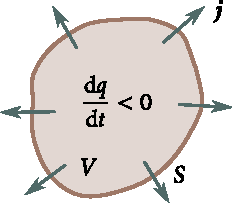
\includegraphics[scale=1]{figures/ch_05/fig_5_1.pdf}
			\caption[]{}
			\label{fig:5_1}
		\end{center}
	\end{minipage}
	\hfill{ }%space{-0.05cm}
	\begin{minipage}[t]{0.48\linewidth}
		\begin{center}
			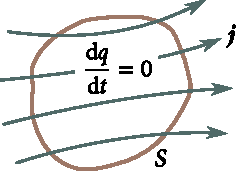
\includegraphics[scale=1]{figures/ch_05/fig_5_2.pdf}
			\caption[]{}
			\label{fig:5_2}
		\end{center}
	\end{minipage}
\vspace{-0.4cm}
\end{figure}

Thay $q$ bằng $\int_V \rho\,\deriv{V}$, ta có phương trình
\begin{equation}\label{eq:5_9}
    \oint_S \vec{j} \ccdot \deriv{\vec{S}} = - \diff{}{t} \int_V \rho\, \deriv{V} = - \int_V \diffpartial{\rho}{t}\, \deriv{V}.
\end{equation}

\noindent
Chúng tôi đã viết đạo hàm riêng của $\rho$ theo $t$ bên trong tích phân vì mật độ điện tích khối có thể
không chỉ phụ thuộc vào thời gian, mà còn vào  
tọa độ (tích phân $\int_V \rho\,\deriv{V}$ là một hàm chỉ phụ thuộc vào thời gian). Chúng ta hãy biến đổi vế trái của \eqn{5_9} theo định lý Ostrogradsky-Gauss. Kết quả là, ta nhận được
\begin{equation}\label{eq:5_10}
    \int_V (\divop{\vec{j}})\, \deriv{V} = - \int_V \diffpartial{\rho}{t}\, \deriv{V}.
\end{equation}

\noindent
Phương trình \eqref{eq:5_10} cần phải được chú ý khi lựa chọn thể tích $V$ tùy ý để lấy tích phân. Điều này chỉ có thể thực hiện được nếu tại mọi điểm trong không gian, điều kiện sau được thỏa mãn 
\begin{equation}\label{eq:5_11}
    \divop{\vec{j}} = - \diffpartial{\rho}{t}.
\end{equation}

\noindent
Phương trình \eqref{eq:5_11} được gọi là \textbf{phương trình liên tục}. Nó [giống \eqn{5_9}] phát biểu định luật bảo toàn điện tích. Dựa vào \eqn{5_11}, điện tích giảm dần tại các điểm là nguồn của vector $\vec{j}$.

Đối với một dòng điện không đổi, điện thế, mật độ điện tích và các đại lượng khác tại các điểm khác nhau là không đổi. Do đó, đối với dòng điện không đổi, \eqn{5_11} có dạng
\begin{equation}\label{eq:5_12}
    \divop{\vec{j}} = 0.
\end{equation}

\noindent
Vì thế, đối với dòng điện không đổi, vector $\vec{j}$ không có khởi điểm. Điều này có nghĩa là các dòng điện không có điểm bắt đầu và kết thúc. Vì vậy, các đường của dòng điện không đổi luôn kín. Theo đó, $\oint_S\vec{j}\ccdot\deriv{\vec{S}}$ bằng không. Do đó, đối với dòng điện không đổi, hình tương tự như \fig{5_1} có dạng được hiển thị trong \fig{5_2}.

\section{Suất điện động}\label{sec:5_3}

Nếu một điện trường được thiết lập trong một vật dẫn và không có biện pháp nào được thực hiện để duy trì nó thì chuyển động của các hạt tải điện rất nhanh sẽ dẫn đến sự biến mất của trường bên trong vật dẫn và ngừng dòng điện. Để duy trì dòng điện trong một thời gian đủ dài, cần phải liên tục loại bỏ khỏi đầu dây dẫn có điện thế thấp hơn (các hạt tải điện được coi là dương) các điện tích do dòng điện mang đến và liên tục cung cấp điện thế cao hơn ở đầu còn lại (\fig{5_3}). Nói cách khác, cần phải luân chuyển các điện tích theo một con đường khép kín. Điều này phù hợp với thực tế là các đường của dòng điện không đổi là khép kín (xem phần trước).

\begin{figure}[!htb]
	\begin{center}
		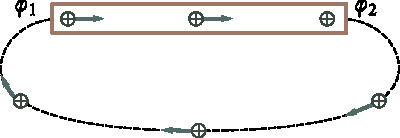
\includegraphics[scale=1]{figures/ch_05/fig_5_3.pdf}
		\caption[]{}
		\label{fig:5_3}
	\end{center}
	\vspace{-0.8cm}
\end{figure}
Lưu số của vector cường độ điện trường bằng không. Do đó, trong một mạch kín, ngoài các phần mà các điện tích dương di chuyển theo chiều giảm của điện thế $\varphi$, phải có các phần mà các điện tích dương di chuyển theo hướng tăng lên của điện thế $\varphi$, tức chống lại các lực của trường tĩnh điện (xem thêm phần mạch điện ở \fig{5_3} được hiển thị bằng đường gạch ngang). Chuyển động của các hạt tải điện trên các phần này chỉ có thể thực hiện được khi có sự hỗ trợ của các lực không có nguồn gốc tĩnh điện, được gọi là \textbf{lực lạ}. Vì vậy, để duy trì dòng điện, các lực lạ cần thiết tác động trên toàn bộ chiều dài của mạch điện hoặc trên các phần riêng biệt của nó. Các lực này có thể là do các quá trình hóa học, sự khuếch tán của các hạt tải điện trong môi trường không đồng nhất hoặc qua mặt phân cách giữa hai chất khác nhau, từ trường biến thiên theo thời gian thiết lập nên điện trường (nhưng không phải trường tĩnh điện) (xem \sect{9_1}),...

% The circulation of the strength vector of an electrostatic field equals zero. Therefore, in a closed circuit, in addition to sections on which the positive carriers travel in the direction of a decrease in the potential $\varphi$, there must be sections on which the positive charges are carried in the direction of a growth in $\varphi$, \ie, against the forces of the electrostatic field (see the part of the circuit in \fig{5_3} shown by the dash line). Motion of the carriers on these sections is possible only with the aid of forces of a non-electrostatic origin, called \textbf{extraneous forces}. Thus, to maintain a current, extraneous forces are needed that act either over the entire length of the circuit or on separate sections of it. These forces may be due to chemical processes, the diffusion of the current carriers in a non-uniform medium or through the interface between two different substances, to electric (but not electrostatic) fields set up by magnetic fields varying with time (see \sect{9_1}), etc.

Các lực lạ có thể được đặc trưng bởi khả năng thực hiện công để dịch chuyển điện tích dọc theo một mạch. Đại lượng bằng công lực lạ thực hiện trên một đơn vị điện tích dương được gọi là \textbf{suất điện động} (viết tắt là \textbf{e.m.f.}) $\mathcal{E}$ trong một đoạn mạch hoặc trên một phần của mạch. Do đó, nếu công của các lực lạ lên điện tích $q$ là $A$ thì
% Extraneous forces can be characterized by the work they do on charges travelling along a circuit. The quantity equal to the work done by the extraneous forces on a unit positive charge is called the \textbf{electromotive force} (\textbf{e.m.f.}) $\mathcal{E}$ acting in a circuit or on a section of it. Hence, if the work of the extraneous forces on the charge $q$ is $A$, then
\begin{equation}\label{eq:5_13}
    \mathcal{E} = \frac{A}{q}.
\end{equation}

So sánh hai phương trình \eqns{1_31}{5_13}, ta thấy suất điện động có cùng thứ nguyên với điện thế. Vì vậy, $\mathcal{E}$ được đo bằng các đơn vị giống như $\varphi$.

Lực lạ $\ab{\vec{F}}{extr}$ tác dụng lên điện tích $q$ có thể được biểu diễn dưới dạng
\begin{equation}\label{eq:5_14}
    \ab{\vec{F}}{extr} = \vec{E}^* q.
\end{equation}

\noindent
Đại lượng vector $\vec{E}^*$ được gọi là \textbf{cường độ điện trường lạ}. Công [của lực lạ tác dụng lên điện tích $q$ trong phần mạch $1$-$2$] là 
\begin{equation*}
    A_{12} = \int_1^2 \ab{\vec{F}}{extr}\, \deriv{\vec{l}} = q \int_1^2 \vec{E}^* \ccdot \deriv{\vec{l}}.
\end{equation*}

\noindent
Chia công này cho $q$, ta được suất điện động trong phần mạch đó:
\begin{equation}\label{eq:5_15}
    \mathcal{E}_{12} = \int_1^2 \vec{E}^* \ccdot \deriv{\vec{l}}.
\end{equation}

\noindent
Một tích phân vòng kín tương tự cho ta suất điện động trong mạch này:
\begin{equation}\label{eq:5_16}
    \mathcal{E} = \oint \vec{E}^* \ccdot \deriv{\vec{l}}.
\end{equation}

\noindent
Do đó, suất điện động trong một mạch kín có thể được xác định như là lưu số của cường độ điện trường lạ.


Ngoài các lực lạ, điện tích còn chịu tác dụng của các lực của trường tĩnh điện $\vec{F}_E=q\vec{E}$.
Vì thế, hợp lực tác dụng tại mỗi điểm của mạch lên điện tích $q$ là
\begin{equation*}
    \vec{F} = \vec{F}_E + \ab{\vec{F}}{extr} = q (\vec{E} + \vec{E}^*).
\end{equation*}

\noindent
Công lực này thực hiện lên điện tích $q$ trong phần mạch $1$-$2$ được xác định bởi biểu thức
\begin{equation}\label{eq:5_17}
    A_{12} = q \int_1^2 \vec{E} \ccdot \deriv{\vec{l}} + q \int_1^2 \vec{E}^* \ccdot \deriv{\vec{l}} = q (\varphi_1 - \varphi_2) + q \mathcal{E}_{12}.
\end{equation}

Đại lượng có giá trị bằng công lực tĩnh điện và lực lạ thực hiện để dịch chuyển một đơn vị điện tích dương được định nghĩa là \textbf{hiệu điện thế} hay đơn giản hơn là \textbf{điện áp} $U$ trong phần xác định của mạch điện. Dựa vào \eqn{5_17},
\begin{equation}\label{eq:5_18}
    U_{12} = \varphi_1 - \varphi_2 + \mathcal{E}_{12}.
\end{equation}

Đoạn mạch không có lực lạ tác dụng gọi là \textbf{thuần nhất}. Đoạn mạch chịu tác dụng của lực lạ gọi là \textbf{không thuần nhất}. Đối với đoạn mạch thuần nhất 
% A section of a circuit on which no extraneous forces act is called \textbf{homogeneous}. A section on which the current carriers experience extraneous forces is called \textbf{inhomogeneous}. For a homogeneous section of a circuit
\begin{equation}\label{eq:5_19}
    U_{12} = \varphi_1 - \varphi_2,
\end{equation}

\noindent
Nghĩa là điện áp trùng với hiệu điện thế giữa hai đầu đoạn mạch.
% \ie, the voltage coincides with the potential difference across the ends of the section.

\section{Định luật Ohm. Điện trở của vật dẫn.}\label{sec:5_4}

Nhà vật lý người Đức Georg Ohm (1789-1854) dựa vào thực nghiệm đã thiết lập một định luật rằng \textit{dòng điện chạy trong vật dẫn kim loại thuần nhất} (tức không có sự tác động của lực lạ) \textit{tỉ lệ thuận với điện áp $U$ đặt lên vật dẫn đó}:
% The German physicist Georg Ohm (1789-1854) experimentally established a law according to which \textit{the current flowing in a homogeneous} (in the meaning that no extraneous forces are present) \textit{metal conductor is proportional to the voltage drop $U$ in the conductor}:
\begin{equation}\label{eq:5_20}
    I = \frac{1}{R} U.
\end{equation}

\noindent
Nhắc lại là đối với vật dẫn thuần nhất, điện áp $U$ bằng hiệu điện thế $\varphi_1-\varphi_2$ [xem \eqn{5_18}].

Đại lượng $R$ trong \eqn{5_20} được gọi là {điện trở} của vật dẫn. Đơn vị của điện trở là ohm (\si{\ohm}) bằng với điện trở của một vật dẫn có dòng điện \SI{1}{\ampere} chạy qua ở điện áp $\SI{1}{\volt}$.

Giá trị của điện trở phụ thuộc vào hình dạng, kích thước của vật dẫn và các đặc tính của vật liệu chế tạo vật dẫn. Đối với dây dẫn hình trụ thuần nhất
\begin{equation}\label{eq:5_21}
    R = \rho \frac{l}{S},
\end{equation}

\noindent
trong đó $l$ là chiều dài dây dẫn, $S$ là tiết diện dây và $\rho$ hệ số phụ thuộc vào đặc tính của vật liệu được gọi là \textbf{điện trở suất}.

Nếu $l=1$ và $S=1$ thì $R$ có giá trị bằng $\rho$. Trong hệ SI, $\rho$ được đo bằng ohm-mét (\si{\ohm\metre}).

Hãy cùng đi tìm liên hệ giữa hai vector $\vec{j}$ và $\vec{E}$ tại cùng một điểm trên vật dẫn. Trong một dây dẫn đẳng hướng, chuyển động có trật tự của các hạt tải điện diễn ra theo hướng của vector $\vec{E}$. Do đó, hướng của hai vector $\vec{j}$ và $\vec{E}$ trùng nhau\footnote{Nói chung, trong các vật thể dị hướng, hướng của các vector $\vec{j}$ và $\vec{E}$ không trùng nhau. Mối liên hệ giữa $\vec{j}$ và $\vec{E}$ đối với các vật thể như vậy được hình thành dưới sự hỗ trợ của tensor độ dẫn điện.}. Chúng ta hãy tính nhẩm thể tích một hình trụ cơ bản có đường sinh song song với hai vector $\vec{j}$ và $\vec{E}$ trong vùng lân cận của một điểm nhất định (\fig{5_4}). Một dòng điện có cường độ bằng $j\,\deriv{S}$ chạy qua tiết diện của hình trụ. Hiệu điện thế đặt vào hình trụ là $E\,\deriv{l}$, trong đó $E$ cường độ điện trường tại điểm đã cho. Cuối cùng, điện trở của hình trụ, dựa vào \eqn{5_21}, là $\rho(\diffin{l}{S})$. Sử dụng các giá trị này trong \eqn{5_21}, ta đi đến phương trình
\begin{equation*}
    j\, \deriv{S} = \frac{1}{\rho} \diff{S}{l} E\, \deriv{l}\quad \text{hay}\quad j = \frac{1}{\rho} E.
\end{equation*}

\noindent
Tận dụng thực tế là các vector $\vec{j}$ và $\vec{E}$ cùng hướng, ta có thể viết
\begin{equation}\label{eq:5_22}
    \vec{j} = \frac{1}{\rho} \vec{E} = \sigma \vec{E}.
\end{equation}

\noindent
Phương trình này biểu diễn định luật Ohm dưới dạng vi phân.

\begin{figure}[!htb]
	\begin{center}
		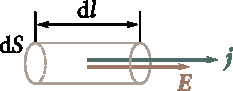
\includegraphics[scale=1]{figures/ch_05/fig_5_4.pdf}
		\caption[]{}
		\label{fig:5_4}
	\end{center}
	\vspace{-0.8cm}
\end{figure}

Đại lượng $\sigma$ trong \eqn{5_22} là nghịch đảo của $\rho$, được gọi là \textbf{độ dẫn điện} của vật liệu. Đơn vị nghịch đảo của ohm được gọi là \textbf{siemens} (\si{\siemens}). Do đó, đơn vị của $\sigma$ là siemens trên mét (\si{\siemens\per\metre}).

Để đơn giản, chúng ta giả sử rằng vật dẫn chứa các hạt tải điện chỉ mang một dấu điện tích. Dựa vào \eqn{5_5}, mật độ dòng điện trong trường hợp này là
\begin{equation}\label{eq:5_23}
    \vec{j} = e n \vec{u}.
\end{equation}

\noindent
So sánh biểu thức này với \eqn{5_22} dẫn chúng ta đến kết luận rằng vận tốc của chuyển động có trật tự của các hạt tải điện tỉ lệ với cường độ điện trường $\vec{E}$, tức tỉ lệ với lực truyền chuyển động có trật tự cho các hạt tải điện. Tỉ lệ thuận giữa vận tốc với lực tác dụng lên vật được quan sát khi ngoài lực tạo ra chuyển động, vật còn chịu thêm lực cản của môi trường. Lực này là do sự tương tác của các hạt tải điện với các phần tử tạo nên vật dẫn. Sự hiện diện của lực cản đối với chuyển động có trật tự của các hạt tải điện gây ra điện trở của vật dẫn.

Khả năng dẫn dòng điện của một chất được đặc trưng bởi điện trở suất $\rho$ hoặc độ dẫn điện $\sigma$. Độ lớn của chúng được xác định bởi bản chất hóa học của chất và các điều kiện xung quanh, cụ thể là nhiệt độ môi trường. 

Điện trở suất $\rho$ thay đổi phụ thuộc trực tiếp vào nhiệt độ tuyệt đối $T$ đối với hầu hết các kim loại ở nhiệt độ gần với nhiệt độ phòng:
\begin{equation}\label{eq:5_24}
    \rho \propto T.
\end{equation}

\noindent
Sự sai lệch so với tỉ lệ này được quan sát thấy ở nhiệt độ thấp (\fig{5_5}). Sự phụ thuộc của $\rho$ vào $T$ thường tuân theo đường cong $1$. Độ lớn của điện trở suất dư $\ab{\rho}{res}$ phụ thuộc rất nhiều vào độ tinh khiết của vật liệu và sự hiện diện của ứng suất cơ dư trong mẫu vật. Đây là lý do tại sao $\ab{\rho}{res}$ giảm đi đáng kể sau khi tôi luyện. Điện trở suất $\rho$ của một kim loại hoàn toàn tinh khiết, có mạng tinh thể cân đối lý tưởng biến mất ở độ không tuyệt đối.
% The magnitude of the residual resistivity $\ab{\rho}{res}$ depends very greatly on the purity of the material and the presence of residual mechanical stresses in the specimen. This is why $\ab{\rho}{res}$ appreciably diminishes after annealing. Điện trở suất $\rho$ of a perfectly pure metal with an ideal regular crystal lattice vanishes at absolute zero. 

\begin{figure}[!htb]
	\begin{center}
		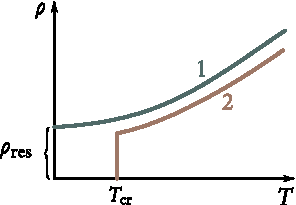
\includegraphics[scale=1]{figures/ch_05/fig_5_5.pdf}
		\caption[]{}
		\label{fig:5_5}
	\end{center}
	\vspace{-0.8cm}
\end{figure}

Điện trở của một nhóm lớn kim loại và hợp kim ở nhiệt độ vài kelvin sẽ biến mất ngay lập tức (đường cong $2$ trong \fig{5_5}). Hiện tượng này, được gọi là \textbf{siêu dẫn}, được phát hiện lần đầu tiên vào năm 1911 bởi nhà khoa học Hà Lan Heike Kamerlingh Onnes (1853-1926) ở thủy ngân. Tính siêu dẫn sau đó được phát hiện trong chì, thiếc, kẽm, nhôm và các kim loại khác, cũng như trong một số hợp kim. Mỗi vật liệu siêu dẫn đều có nhiệt độ tới hạn riêng $\ab{T}{cr}$ mà tại đó nó chuyển sang trạng thái siêu dẫn. Trạng thái siêu dẫn bị can thiệp khi từ trường tác dụng lên chất siêu dẫn. Độ lớn của từ trường tới hạn phá hủy tính siêu dẫn $\ab{B}{cr}$ (kí hiệu $B$ là viết tắt của cảm ứng từ---xem \sect{6_2}) bằng không khi $T=\ab{T}{cr}$ và tăng khi nhiệt độ thấp hơn.

% The resistance of a large group of metals and alloys at a temperature of the order of several kelvins vanishes in a jump (curve $2$ in \fig{5_5}). This phenomenon, called \textbf{superconductivity}, was first discovered in 1911 by the Dutch scientist Heike Kamerlingh Onnes (1853-1926) for mercury. Superconductivity was later discovered in lead, tin, zinc, aluminium, and other metals, as well as in a number of alloys. Every superconductor has its own critical temperature $\ab{T}{cr}$ at which it passes over into a superconducting state. The superconducting state is violated when a magnetic field acts on a superconductor. The magnitude of the critical field $\ab{B}{cr}$ (the symbol $B$ stands for the magnetic induction---see \sect{6_2}) destroying superconductivity equals zero when $T=\ab{T}{cr}$ and grows with lowering of the temperature.
Một chứng minh lý thuyết hoàn chỉnh về hiện tượng siêu dẫn được đưa ra vào năm 1957 bởi J. Bardeen, L. Cooper và J. Schrieffer (xem Vol. III, Sec. 8.2).

Sự phụ thuộc vào nhiệt độ của điện trở làm cơ sở cho việc thiết kế các nhiệt kế điện trở. Một nhiệt kế như vậy là một dây kim loại (thường là bạch kim) được quấn trên thân bằng sứ hoặc mica. Một nhiệt kế điện trở được chia độ theo các điểm nhiệt độ không đổi giúp ta có thể đo cả nhiệt độ thấp và nhiệt độ cao với độ chính xác khoảng vài phần trăm kelvin. Thời gian gần đây, nhiệt kế điện trở bán dẫn ngày càng được ưa chuộng.
% The temperature dependence of resistance underlies the design of resistance thermometers. Such a thermometer is a metal (usually platinum) wire wound onto a porcelain or mica body. A resistance thermometer graduated according to constant temperature points makes it possible to measure both low and high temperatures with an accuracy of the order of several hundredths of a kelvin. Recent times have seen semiconductor resistance thermometers coming into greater and greater favour.

\section{Định luật Ohm cho đoạn mạch không thuần nhất}\label{sec:5_5}

Các lực lạ $e\vec{E}^*$ tác dụng lên các hạt tải điện trên một đoạn mạch không thuần nhất cùng các lực tĩnh điện $e\vec{E}$. Các lực lạ có khả năng tạo ra chuyển động có trật tự của các hạt tải điện ở mức độ tương tự như lực tĩnh điện. Chúng ta đã tìm thấy trong phần trước rằng trong một vật dẫn thuần nhất, vận tốc trung bình của chuyển động có trật tự của các hạt tải điện tỉ lệ với lực tĩnh điện $e\vec{E}$. Khá rõ ràng là ở nơi các lực lạ tác dụng lên các hạt tải điện cùng với lực tĩnh điện, vận tốc trung bình của chuyển động có trật tự của các hạt tải điện sẽ tỉ lệ với tổng lực $e\vec{E}+ e\vec{E}^*$. Theo đó, mật độ dòng điện tại các điểm này tỉ lệ thuận với tổng các cường độ trường
% The extraneous forces $e\vec{E}^*$ act on current carriers on an inhomogeneous section of a circuit in addition to the electrostatic forces $e\vec{E}$. Extraneous forces are capable of producing ordered motion of current carriers to the same extent as electrostatic forces are. We found in the preceding section that in a homogeneous conductor, the average velocity of ordered motion of the current carriers is proportional to the electrostatic force $e\vec{E}$. It is quite obvious that, where extraneous forces are exerted on the carriers in addition to the electrostatic forces, the average velocity of ordered motion of the carriers will be proportional to the total force $e\vec{E}+ e\vec{E}^*$. Accordingly, the current density at these points is proportional to the sum of the strengths $\vec{E}+\vec{E}^*$:
\begin{equation}\label{eq:5_25}
    \vec{j} = \sigma \parenthesis{\vec{E}+\vec{E}^*}.
\end{equation}

Phương trình \eqref{eq:5_25} tóm tắt \eqn{5_22} đối với một vật dẫn không thuần nhất. Nó biểu diễn định luật Ohm cho phần mạch không thuần nhất dưới dạng vi phân.

Chúng ta có thể chuyển định luật Ohm từ dạng vi phân sang dạng tích phân. Chúng ta hãy xem xét một đoạn mạch không thuần nhất. Giả sử rằng có một đường bên trong phần này (chúng ta sẽ gọi nó là đường dẫn điện) tuân theo các điều kiện sau: ($1$) trong mọi mặt cắt vuông góc với đường dẫn, các đại lượng $\vec{j}$, $\sigma$, $\vec{E}$, $\vec{E}^*$ có các giá trị giống nhau với đủ độ chính xác và ($2$) các vector $\vec{j}$, $\vec{E}$ và $\vec{E}^*$ tại mọi điểm đều hướng theo tiếp tuyến của đường dẫn. Tiết diện của dây dẫn có thể thay đổi (\fig{5_6}).
% We can pass over from Ohm's law in the differential form to its integral form. Let us consider an inhomogeneous section of a circuit. Assume that there is a line inside this section (we shall call it the current path) complying with the following conditions: ($1$) in every cross section perpendicular to the path, the quantities $\vec{j}$, $\sigma$, $\vec{E}$, $\vec{E}^*$ have the same values with sufficient accuracy, and ($2$) the vectors $\vec{j}$, $\vec{E}$, and $\vec{E}^*$ at every point are directed along a tangent to the path. The cross section of the conductor may vary (\fig{5_6}).

\begin{figure}[!htb]
	\begin{center}
		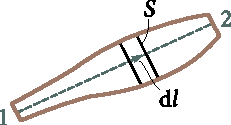
\includegraphics[scale=1]{figures/ch_05/fig_5_6.pdf}
		\caption[]{}
		\label{fig:5_6}
	\end{center}
	\vspace{-0.8cm}
\end{figure}

Chúng ta hãy chọn một hướng chuyển động tùy ý dọc theo đường dẫn. Giả sử rằng hướng đã chọn trong \fig{5_6} tương ứng với chuyển động từ đầu $1$ đến đầu $2$ của đoạn mạch (hướng $1$-$2$). Chiếu các vector trong \eqn{5_25} lên phần tử đường dẫn $\deriv{\vec{l}}$. Kết quả là
% Let us choose an arbitrary direction of motion along the path. Assume that the chosen \fig{5_6} direction corresponds to motion from end $1$ to end $2$ of the circuit section (direction $1$-$2$). Let us project the vectors in \eqn{5_25} onto the path element $\deriv{\vec{l}}$. The result is
\begin{equation}\label{eq:5_26}
    j_l = \sigma (E_l + E_l^*).
\end{equation}

\noindent
Nhờ vào các giả thiết của chúng ta, hình chiếu của mỗi vector bằng độ lớn của vector đó và nhận dấu dương hay âm tùy thuộc vào hướng của vector đó so với $\deriv{\vec{l}}$. Ví dụ, $j_l=j$ nếu dòng điện chạy theo hướng $1$-$2$ và $j_l=-j$ nếu dòng điện chạy theo hướng $2$-$1$.
% Owing to our assumption, the projection of each of the vectors equals the magnitude of the vector taken with the sign plus or minus depending on the direction of the vector relative to $\deriv{\vec{l}}$. For example, $j_l=j$ if the current flows in direction $1$-$2$, and $j_l=-j$ if it flows in direction $2$-$1$.

Do sự bảo toàn điện tích, dòng điện không đổi trong mỗi phần phải giống nhau. Do đó, đại lượng $I=j_lS$ là không đổi dọc theo đường dẫn. Dòng điện trong trường hợp này nên được xem như một đại lượng mang giá trị đại số. Hãy nhớ rằng ta đã chọn hướng $1$-$2$ một cách tùy ý. Vì thế, nếu dòng điện chạy theo hướng đã chọn, nó sẽ được xem là dương và nếu nó chạy theo hướng ngược lại (tức từ đầu $2$ đến đầu $1$) thì được xem là âm.


Hãy dùng tỉ lệ $I/S$ thay thế cho $j_l$ và điện trở suất $\rho$ thay thế cho độ dẫn điện $\sigma$ trong \eqn{5_26}. Ta được
\begin{equation*}
    I \frac{\rho}{S} = E_l + E_l^*.
\end{equation*}

\noindent
Nhân phương trình trên với $\deriv{l}$ và tích phân theo đường dẫn
\begin{equation*}
    I \int_1^2 \rho\, \frac{\deriv{l}}{S} = \int_1^2 E_l\, \deriv{l} + \int_1^2 E_l^*\, \deriv{l}.
\end{equation*}

\noindent
Đại lượng $\rho(\deriv{l}/S)$ là điện trở của đoạn đường dẫn có độ dài $\deriv{l}$ và tích phân của đại lượng này là điện trở $R$ của đoạn mạch. Tích phân đầu tiên ở vế phải cho $\varphi_1-\varphi_2$ và tích phân thứ hai cho suất điện động $\mathcal{E}_{12}$ đặt vào đoạn mạch. Do đó, ta đi đến phương trình
\begin{equation}\label{eq:5_27}
    I R = \varphi_1 - \varphi_2 + \mathcal{E}_{12}.
\end{equation}

Suất điện động $\mathcal{E}_{12}$, như cường độ dòng điện $I$, là một đại mang giá trị đại số. Nếu suất điện động này tạo điều kiện cho chuyển động của các hạt tải điện dương theo hướng đã chọn (hướng $1$-$2$), ta có $\mathcal{E}_{12}>0$. Còn nếu suất điện động này ngăn cản chuyển động của các hạt tải điện dương theo hướng đã cho, $\mathcal{E}_{12}<0$.

Hãy viết \eqn{5_27} dưới dạng
\begin{equation}\label{eq:5_28}
    I= \frac{\varphi_1 - \varphi_2 + \mathcal{E}_{12}}{R}.
\end{equation}

\noindent
Phương trình này biểu diễn định luật Ohm cho một đoạn mạch không thuần nhất. Giả sử rằng $\varphi_1=\varphi_2$, ta nhận được phương trình của định luật Ohm cho một mạch kín:
\begin{equation}\label{eq:5_29}
    I= \frac{\mathcal{E}}{R}.
\end{equation}

\noindent
Ở đây, $\mathcal{E}$ là suất điện động được đặt vào mạch điện và $R$ là tổng trở của toàn mạch.

\section{Mạch đa vòng. Định luật Kirchhoff}\label{sec:5_6}

Việc tính toán các mạng hoặc mạch đa vòng sẽ đơn giản đáng kể nếu chúng ta sử dụng hai định luật do nhà vật lý người Đức Gustav Kirchhoff (1824-1887) xây dựng. Định luật đầu tiên liên quan đến các nút mạng. Một \textbf{nút} được định nghĩa là giao điểm của ba dây dẫn trở lên (\fig{5_7}). Dòng điện chạy về phía nút mạng được xem là mang một dấu (cộng hoặc trừ) và dòng điện chạy ra xa nút mạng sẽ mang dấu ngược lại (trừ hoặc cộng).

% \begin{figure}[t]
% 	\begin{center}
% 		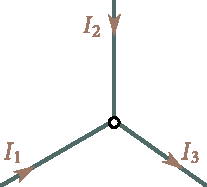
\includegraphics[scale=1]{figures/ch_05/fig_5_7.pdf}
% 		\caption[]{}
% 		\label{fig:5_7}
% 	\end{center}
% 	\vspace{-0.8cm}
% \end{figure}

\begin{figure}[!htb]
	\begin{minipage}[t]{0.38\linewidth}
		\begin{center}
			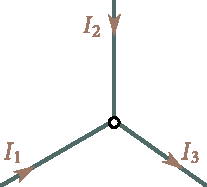
\includegraphics[scale=1]{figures/ch_05/fig_5_7.pdf}
			\caption[]{}
			\label{fig:5_7}
		\end{center}
	\end{minipage}
	\hfill{ }%space{-0.05cm}
	\begin{minipage}[t]{0.58\linewidth}
		\begin{center}
			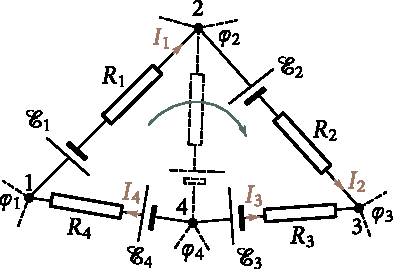
\includegraphics[scale=1]{figures/ch_05/fig_5_8.pdf}
			\caption[]{}
			\label{fig:5_8}
		\end{center}
	\end{minipage}
\vspace{-0.4cm}
\end{figure}

Định luật Kirchhoff đầu tiên, còn được gọi là \textbf{định luật nút}, phát biểu rằng \textit{tổng đại số của tất cả các dòng điện đi vào một nút phải bằng không}:
\begin{equation}\label{eq:5_30}
    \sum_k I_k = 0.
\end{equation}

\noindent
Định luật này tuân theo phương trình liên tục, tức là hệ quả của định luật bảo toàn điện tích. Đối với một dòng điện không đổi, $\divop{\vec{j}}$ bằng không tại mọi điểm [xem \eqn{5_21}]. Do đó, thông lượng của vector $\vec{j}$ hay tổng đại số của các dòng điện chạy qua một mặt kín tưởng tượng bao quanh một nút phải bằng không.
% This rule follows from the continuity equation, \ie, in the long run from the law of charge conservation. For a steady current, $\divop{\vec{j}}$ equals zero everywhere [see \eqn{5_21}]. Hence, the flux of the vector $\vec{j}$, \ie, the algebraic sum of the currents flowing through an imaginary closed surface surrounding a junction, must be zero.

Phương trình \eqref{eq:5_30} có thể được viết cho mỗi nút trong $N$ nút mạng. Tuy nhiên, chỉ có $N-1$ phương trình là độc lập còn phương trình thứ $N$ sẽ là một hệ quả của hệ phương trình trên.

Định luật thứ hai liên quan đến bất kỳ vòng kín nào được lấy ra từ mạch đa vòng (ví dụ: xem vòng lặp $1$-$2$-$3$-$4$-$1$ trong \fig{5_8}). Chọn một chiều mắt mạng bất kì (ví dụ, theo chiều kim đồng hồ như trong hình) và áp dụng định luật Ohm cho mỗi vòng không phân nhánh:
% The second rule relates to any closed loop separated from a multiloop circuit (see, for example, loop $1$-$2$-$3$-$4$-$1$ in \fig{5_8}). Let us choose a direction of circumvention (for example, clockwise as in the figure) and apply Ohm's law to each unbranched loop section:
\begin{align*}
    I_1 R_1 &= \varphi_1 - \varphi_2 + \mathcal{E}_1\\
    I_2 R_2 &= \varphi_2 - \varphi_3 + \mathcal{E}_2\\
    I_3 R_3 &= \varphi_3 - \varphi_4 + \mathcal{E}_3\\
    I_4 R_4 &= \varphi_4 - \varphi_1 + \mathcal{E}_4.
\end{align*}

\noindent
Khi tính tổng các biểu thức này, các điện thế sẽ bị triệt tiêu và ta có phương trình
\begin{equation}\label{eq:5_31}
    \sum_k I_k R_k = \sum_k \mathcal{E}_k,
\end{equation}

\noindent
phát biểu \textbf{Định luật Kirchhoff 2}, còn được gọi là \textbf{định luật mắt mạng}.

% \begin{figure}[t]
% 	\begin{center}
% 		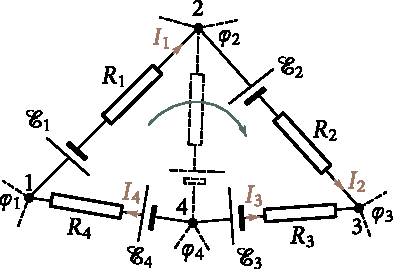
\includegraphics[scale=1]{figures/ch_05/fig_5_8.pdf}
% 		\caption[]{}
% 		\label{fig:5_8}
% 	\end{center}
% 	\vspace{-0.8cm}
% \end{figure}

Phương trình \eqref{eq:5_31} có thể được viết cho tất cả các vòng kín có thể tách ra được từ một mạch điện đa vòng nhất định. Tuy nhiên, chỉ những phương trình cho các vòng không được tạo nên bằng việc chồng các vòng khác lên nhau thì mới độc lập. Ví dụ, đối với mạch điện được mô tả trong \fig{5_9}, ta có thể viết được ba phương trình:
% Only the equations for the loops that cannot be obtained by the superposition of other loops on one another will be independent, however. For example, for the circuit depicted in \fig{5_9}, we can write three equations:
\begin{enumerate}[(1)]
    \item cho vòng $1$-$2$-$3$-$6$-$1$,
    \item cho vòng $3$-$4$-$5$-$6$-$3$, và
    \item cho vòng $1$-$2$-$3$-$4$-$5$-$6$-$1$.
\end{enumerate}

Vòng cuối cùng có được bằng cách chồng hai vòng đầu tiên. Vì vậy, các phương trình sẽ không độc lập. Chúng ta có thể coi hai phương trình bất kỳ trong ba phương trình đó là độc lập.

Khi viết phương trình của định luật mắt mạng, chúng ta phải chỉ định các dấu của dòng điện và suất điện động phù hợp với chiều dương đã chọn. Ví dụ, dòng điện $I_1$ trong \fig{5_9} phải âm vì nó đi ngược lại với chiều dương đã chọn. Suất điện động cũng âm vì nó hoạt động ngược chiều dương...
% In writing the equations of the loop rule, we must appoint the signs of the currents and e.m.f.'s in accordance with the chosen direction of circumvention. For example, the current $I_1$ in \fig{5_9} must be considered negative because it flows oppositely to the chosen direction of circumvention. The e.m.f. must also be considered negative because it acts in the direction opposite to that of circumvention, and so on.

Chúng ta có thể chọn chiều dương trong mỗi vòng hoàn toàn tùy ý và độc lập với các cách chọn chiều dương trong các vòng khác. Ở đây, có thể xảy ra trường hợp rằng cùng một dòng điện hoặc cùng một suất điện động có thể được đưa vào các phương trình khác nhau với các dấu trái ngược nhau (điều này xảy ra với dòng điện $I_2$ trong \fig{5_9} khi xem xét các chiều dương được chỉ định trong các vòng). Tuy nhiên, điều này không có ý nghĩa gì vì sự thay đổi hướng xung quanh một vòng chỉ dẫn đến sự đảo ngược của tất cả các dấu trong \eqn{5_31}.
% We may choose the direction of circumvention in each loop absolutely arbitrarily and independently of the choice of the directions in the other loops. It may happen, here, that the same current or the same e.m.f. may be included in different equations with opposite signs (this happens with the current $I_2$ in \fig{5_9} for the indicated directions of circumvention in the loops). This is of no significance, however, because a change in the direction around a loop results only in a reversal of all the signs in \eqn{5_31}.

\begin{figure}[!htb]
	\begin{center}
		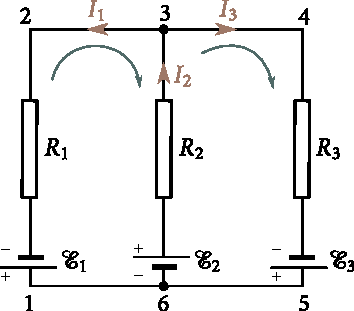
\includegraphics[scale=1]{figures/ch_05/fig_5_9.pdf}
		\caption[]{}
		\label{fig:5_9}
	\end{center}
	\vspace{-0.8cm}
\end{figure}

Khi viết các phương trình, hãy nhớ rằng dòng điện chạy trong bất kì tiết diện nào của phần mạch không phân nhánh là như nhau. Ví dụ, cùng một dòng điện $I_2$ chạy từ nút $6$ đến nguồn điện $\mathcal{E}_2$ cũng như từ nguồn $\mathcal{E}_2$ đến nút $3$.

Số lượng các phương trình độc lập được viết dựa theo định luật nút và vòng bằng số dòng điện phân biệt chạy trong một mạch đa vòng. Vì vậy, nếu ta biết suất điện động và điện trở của tất cả các đoạn mạch không phân nhánh, ta có thể tính được tất cả các dòng điện. Ta cũng có thể giải quyết các vấn đề khác, chẳng hạn như tìm các suất điện động được đặt vào mỗi đoạn mạch để có dòng điện cần thiết với các điện trở đã cho.
% The number of independent equations compiled in accordance with the junction and loop rules equals the number of different currents flowing in a multiloop circuit. Therefore, if we know the e.m.f.'s and resistances for all the unbranched sections, we can calculate all the currents. We can also solve other problems, for instance find the e.m.f.'s that must be connected in each of the sections of a circuit to obtain the required currents with the given resistances.

\section{Công suất của dòng điện}\label{sec:5_7}

Hãy phân tích một đoạn mạch bất kì có dòng điện không đổi chạy qua và điện áp $U$ được đặt vào hai đầu của nó. Lượng điện tích $q=It$ chạy qua mọi tiết diện của dây dẫn trong thời gian $t$. Điều này tương đương với thực tế là lượng điện tích $It$ được truyền từ đầu này sang đầu khác của dây dẫn trong thời gian $t$. Lực tĩnh điện và lực lạ tác dụng lên đoạn mạch thực hiện công
%Let us consider an arbitrary section of a steady current circuit across whose ends the voltage $U$ is applied. The charge $q=It$ will flow during the time $t$ through every cross section of the conductor. This is equivalent to the fact that the charge $It$ is carried during the time $t$ from one end of the conductor to the other. The forces of the electrostatic field and the extraneous forces acting on the given section do the work
\begin{equation}\label{eq:5_32}
    A = U q = U I t
\end{equation}

\noindent
[nhắc lại rằng điện áp $U$ được định nghĩa là công lực điện và lực lạ thực hiện để dịch chuyển một đơn vị điện tích dương; xem \eqn{5_18}].

Chia công $A$ cho thời gian thực hiện công $t$, ta được công suất dòng điện thực hiện trên đoạn mạch đang xét:
\begin{equation}\label{eq:5_33}
    P = U I = (\varphi_1 - \varphi_2) I + \mathcal{E}_{12} + I.
\end{equation}

\noindent
Công suất này có thể được chuyển hóa thành công do mạch ngoài thực hiện (để làm được như vậy, mạch điện phải dịch chuyển trong không gian) hay để tiến hành các phản ứng hóa học hoặc làm tăng nhiệt độ cho mạch đó.

Tỉ số giữa công suất $\Delta{P}$ do dòng điện sinh ra trong thể tích $\Delta{V}$ của dây dẫn với độ lớn của thể tích đó được gọi là \textbf{công suất đơn vị của dòng điện} $\ab{P}{u}$, tương ứng với điểm đang xét của dây dẫn. Theo định nghĩa trên, công suất đơn vị có công thức 
%The ratio of the power $\Delta{P}$ developed by a current in the volume $\Delta{V}$ of a conductor to the magnitude of this volume is called the \textbf{unit power of the current} $\ab{P}{u}$, corresponding to the given point of the conductor. By definition, the unit power is
\begin{equation}\label{eq:5_34}
    \ab{P}{u} = \frac{\Delta{P}}{\Delta{V}}.
\end{equation}

\noindent
Nói cách khác, công suất đơn vị là công suất trên một đơn vị thể tích của dây dẫn.
%Speaking conditionally, the unit power is the power developed in unit volume of a conductor.

Biểu thức cho công suất đơn vị có thể được thiết lập từ những lập luận sau đây. Lực $e(\vec{E}+\vec{E}^*)$ tạo ra một công suất
%An expression for the unit power can be obtained proceeding from the following considerations. The force $e(\vec{E}+\vec{E}^*)$ develops a power of
\begin{equation*}
    P' = e (\vec{E} + \vec{E}^*) (\vec{v} + \vec{u})
\end{equation*}

\noindent
dựa trên chuyển động của hạt tải điện. Hãy lấy giá trị trung bình biểu thức này cho các hạt tải điện bị giới hạn trong thể tích $\Delta{V}$ mà trong đó $\vec{E}$ và $\vec{E}^*$ xem như không đổi. Kết quả là
%upon the motion of a current carrier. Let us average this expression for the carriers confined in the volume $\Delta{V}$ within which $\vec{E}$ and $\vec{E}^*$ may be considered constant. The result is
\begin{equation*}
    \average{P'} = e (\vec{E} + \vec{E}^*) \average{\vec{v} + \vec{u}} = e (\vec{E} + \vec{E}^*) \average{\vec{v}} + e (\vec{E} + \vec{E}^*) \average{\vec{u}} = e (\vec{E} + \vec{E}^*) \average{\vec{u}}
\end{equation*}

\noindent
(hãy nhớ rằng $\average{\vec{v}}=0$).

Ta có thể xác định công suất $\Delta{P}$ được thực hiện trong thể tích $\Delta{V}$ bằng cách nhân $\average{P'}$ với số lượng hạt tải điện bên trong thể tích đó, nghĩa là bằng $n\Delta{V}$ ($n$ số hạt tải điện trong thể tích đơn vị). Do đó,
\begin{equation*}
    \Delta{P} = \average{P'} n \Delta{V} = e (\vec{E} + \vec{E}^*) \ccdot \average{\vec{u}} n \Delta{V} = \vec{j} \ccdot (\vec{E} + \vec{E}^*) \Delta{V}
\end{equation*}

\noindent
[xem \eqn{5_23}]. Từ đây,
\begin{equation}\label{eq:5_35}
    \ab{P}{u} = \vec{j} \ccdot (\vec{E} + \vec{E}^*)
\end{equation}

\noindent
Biểu thức này là một dạng vi phân của tích phân \eqref{eq:5_33}.

\section{Định luật Joule-Lenz}\label{sec:5_8}

Khi một vật dẫn đứng yên và không có biến đổi hóa học nào xảy ra bên trong nó, thì công của dòng điện được cho bởi \eqn{5_32} sẽ làm tăng nội năng của vật dẫn và kết quả là vật dẫn đó bị nóng lên. Thông thường người ta nói rằng khi dòng điện chạy trong vật dẫn thì nhiệt lượng
%When a conductor is stationary and no chemical transformations occur in it, the work of a current given by \eqn{5_32} goes to increase the internal energy of the conductor, and as a result the latter gets heated. It is customary to say that when a current flows in a conductor, the heat
\begin{equation*}
    Q = U I t
\end{equation*}

\noindent
tỏa ra. Thay $U$ bằng $RI$ theo định luật Ohm, ta được biểu thức
\begin{equation}\label{eq:5_36}
    Q = R I^2 t.
\end{equation}

Phương trình \eqref{eq:5_36} được thiết lập bằng thực nghiệm độc lập bởi nhà vật lý người Anh James Joule (1818-1889) và nhà vật lý người Nga Emil Lenz (1804 1865), và nó được gọi là \textbf{định luật Joule-Lenz}.

Nếu cường độ dòng điện thay đổi theo thời gian thì nhiệt lượng tỏa ra trong thời gian $t$ được tính bằng phương trình
\begin{equation}\label{eq:5_37}
    Q = \int_0^t R I^2\, \deriv{t}.
\end{equation}

Chúng ta có thể chuyển từ phương trình xác định nhiệt lượng tỏa ra trên toàn bộ dẫn \eqn{5_36} sang một biểu thức đặc trưng cho sự tỏa nhiệt tại các điểm khác nhau của vật dẫn. Hãy tách ra từ vật dẫn, như cách chúng ta đã làm trong việc suy luận ra \eqn{5_22}, một thể tích hình trụ cơ bản (xem \fig{5_4}). Theo định luật Joule-Lenz, nhiệt lượng dưới đây sẽ được tỏa ra trên thể tích này trong thời gian $\deriv{t}$:
%We can pass over from \eqn{5_36} determining the heat liberated in an entire conductor to an expression characterizing the liberation of heat at different spots of the conductor. Let us separate in a conductor, in the same way as we did in deriving \eqn{5_22}, an elementary volume in the form of a cylinder (see \fig{5_4}). According to the Joule-Lenz law, the following amount of heat will be liberated in this volume during the time $\deriv{t}$:
\begin{equation}\label{eq:5_38}
    \deriv{Q} = R I^2\, \deriv{t} = \frac{\rho\, \deriv{l}}{\deriv{S}} (j\, \deriv{S})^2\, \deriv{t} = \rho j^2\, \deriv{V}\, \deriv{t}
\end{equation}

\noindent
($\deriv{V}=\deriv{S}\, \deriv{l}$ là độ lớn của thể tích cơ bản).

Chia \eqn{5_38} cho $\deriv{V}$ và $\deriv{t}$, ta sẽ tính được nhiệt lượng tỏa ra trên một đơn vị thể tích trong một đơn vị thời gian:
\begin{equation}\label{eq:5_39}
    \ab{Q}{u} = \rho j^2.
\end{equation}

\noindent
Tương tự với tên của đại lượng \eqn{5_34},đại lượng $\ab{Q}{u}$ có thể được gọi là \textbf{nhiệt năng đơn vị của dòng điện}.

Phương trình \eqref{eq:5_39} là một dạng vi phân của định luật Joule-Lenz. có thể được suy ra từ \eqn{5_35}. Sử dụng $\vec{j}/\sigma= \rho\vec{j}$ thay cho $\vec{E}+\vec{E}^*$ trong \eqn{5_35} [xem \eqn{5_25}], ta được phương trình 
\begin{equation*}
    \ab{P}{u} = \rho \vec{j}^2,
\end{equation*}

\noindent
trùng khớp với \eqn{5_39}.

Cần phải lưu ý rằng Joule và Lenz đã thiết lập định luật của họ cho một đoạn mạch thuần nhất. Tuy nhiên, theo như những gì đã nói trong mục này, \eqns{5_36}{5_39} cũng có tác dụng đối với phần không thuần nhất với điều kiện là các lực lạ tác dụng lên nó có nguồn gốc phi hóa học.

